\documentclass[a4paper,11pt]{article}

\parindent0cm
\usepackage
[backend=biber,style=apa,sorting=nyt]
{biblatex}
\addbibresource{literature.bib}

\usepackage[utf8]{inputenc}
\usepackage{csquotes}
\usepackage{array}
\usepackage{dirtytalk}
\usepackage{amsmath}
\usepackage{amssymb}
\usepackage{amsthm}
\usepackage{amsfonts}
\usepackage{color}
\usepackage{layouts}
% printing the textsize used
% \printinunitsof{cm}
% \prntlen{\textwidth}
\usepackage[usenames,dvipsnames]{xcolor}
\usepackage{tabularx}
\usepackage{graphicx}
\usepackage{pdfpages}
\usepackage[ngerman]{babel}
\usepackage[left=3cm,right=2.5cm,top=2cm,bottom=2cm]{geometry}
\renewcommand{\baselinestretch}{1.5}\normalsize % Zeilenabstand 1.5



\begin{document}

\begin{titlepage}

\vspace*{3cm}


\begin{figure}[t]
\begin{flushright}
\includegraphics[width = 7cm,  keepaspectratio]{Images/TULogo.png}
\label{fig2}

\end{flushright}
\end{figure}
\vspace*{3cm}


\begin{center}

\vspace*{2cm}

\title{Masterthesis}



{\huge Masterthesis}\\
 {\huge{\textbf{Multilabel-Klassifizierung \\
 von Nachrichten Schlagzeilen}}\\}
 \vspace{0.2cm}
 {\large  Vergleich zwischen neuronalen Netzen und baumbasierten Algorithmen auf verschiedenen Repräsentationen von Wörtern\\}
\vspace*{5cm}


{\large  Fakultät Statistik\\
Lehrstuhl Statistical Methods for Big Data }
\vspace*{0.5cm}

 \begin{large}
 Betreuer: Prof. Dr. Andreas Groll\\
  \end{large}

  \begin{large}
Verfasser: Marc Schmieder\\
\date{October 2019}
   \vspace*{2cm}

 \end{large}
\end{center}
\newpage
%\large
\thispagestyle{empty}
\tableofcontents
\newpage
\end{titlepage}







\section{Einleitung}

\begin{itemize}
    \item nutzen der klassifikation für die Redaktion
    \item oft nur binäre klassifikation, multi selteneres topic
    \item multiclass auch bei next best offer
    \item bag of words kein guten Ruf, bei welchen Datensätzen lohnen sich Neural nets überhaupt.
\end{itemize}{}

\section{Datensatz und Problemstellung}

In diesem Kapitel wird der für diese Thesis relevante Datensatz vorgestellt. Nach dessen Bereinigung erfolgt eine Exploration und anschließend die Darlegung der Zielstellung dieser Thesis.


\subsection{Initialer Datensatz}

Der Datensatz trägt den Titel \textit{News Category Dataset} (\cite{dataset}) und stammt von der Machine Learning Plattform \textit{Kaggle}. Er umfasst $200853$ Beobachtungen, die Informationen in englischer Sprache über Artikel der US-Amerikanischen Onlinezeitung \textit{Huffpost} enthalten. Der Zeitraum, in dem die Veröffentlichungen stattgefunden haben, erstreckt sich vom 28.01.2012 bis zum 25.05.2018, also über eine Zeitspanne von über $6$ Jahren. Die Inhalte der Artikel sind lediglich verlinkt und nicht direkt im Datensatz enthalten. Für jeden Artikel ist die Nachrichtenschlagzeile des Artikels angegeben. Zusätzlich zu dem Link des Artikels ist für jeden Datenpunkt das Veröffentlichungsdatum, der Name des Autors, eine Kurzbeschreibung und die Nachrichtenkategorie gegeben. Letzteres ist die Zielvariable (genauere Erläuterung in Kapitel \ref{Kap:Zielst}), die $41$ verschiedene Ausprägungen annimmt. Die Kurzbeschreibung enthält ähnliche Informationen wie die Nachrichtenüberschrift und ist nur teilweise vorhanden. Für die Beantwortung der Fragestellung (Kapitel \ref{Kap:Zielst}) soll nur die Schlagzeile als abhängige Variable in die Modellierung eingehen. Bevor eine Exploration des Datensatz erfolgt, werden im nächsten Abschnitt vorgenommene Änderungen an den relevanten Spalten Nachrichtenkategorie und Nachrichtenschlagzeile aufgelistet und begründet.


\subsection{Änderungen am Datensatz} \label{kap:2_2Aend}

In der US-amerikanischen Sprache spielt die Groß- und Kleinschreibung außer bei der Nutzung von Personalpronomen keine Rolle. Deshalb wurden in den Texten alle Großbuchstaben zu Kleinbuchstaben konvertiert. Auf diese Weise werden in der Modellierung beispielsweise die Wörter \textit{Teacher} und \textit{teacher} nicht unterschiedlich behandelt. \\
\\
Die Artikel wurden vermutlich von einigen Autoren in unterschiedlichen Ländern geschrieben, denn die Texte enthalten unterschiedliche Zeichensätze. Bei der verwendeten \texttt{utf8} Enkodierung entstanden bei unbekannten Zeichen Konvertierungsfehler (z.b. der Form \say{a@S}). Diese wurden durch Leerzeichen ersetzt. In dem Wissen, dass die Wörter des Textkorpus mit den \textit{Global Word Vectors} (Kapitel \ref{Kap:Glove}) abgeglichen werden, wurden einige Begriffe so ersetzt, dass bestimmte Wörter in den \textit{Global Word Vectors} gefunden werden. Zuerst erfolgte eine Entfernung von Sonderzeichen wie beispielsweise \say{©} oder \say{™}. Dann folgte die Ersetzung von Verneinungen wie zum Beispiel \say{n't} durch \say{ not}. Analog wurden \say{'ll} durch \say{ will} und \say{'ve} durch \say{ have} ersetzt. Kurzformen der Form \say{here's} wurden zu \say{here is} geändert, da sonst die Wörter mit Endung \say{'s} so als eigenständige Wörter repräsentiert werden und nicht sinngemäß als Tupel. Häufig vorkommende Eigennamen mit analoger Endung \say{trump's} wurden durch \say{trump his} ausgetauscht. Nachdem Vorkommnisse der Art \say{here's} entfernt worden, können nun Vorkommnisse der Art \say{john's son} durch \say{john its son} ersetzt werden. So ist bei Wörtertupeln dieser Art zwar nicht das Geschlecht von John bekannt, aber zumindest offensichtlich, dass der Sohn John zugehörig ist. Nach der Bereinigung des Textkorpus wurden letztendlich noch $6$ Schlagzeilen entfernt, die keine Wörter mehr enthalten. Es verbleiben nun also insgesamt $200847$ Beobachtungen.\\
\\
Nach der umfangreichen Bereinigung des Schlagzeilen-Textkorpuses liegt nun die Zielvariable Nachrichtenkategorie im Fokus.
Bei genauerer Betrachtung der $41$ Kategorien fällt auf, dass diese teilweise bereits namentlich sehr ähnlich ausfallen. In Tabelle \ref{tab:parentsMerge} sind beispielhaft $4$ Schlagzeilen der Kategorien \textit{parents} und \textit{parenting} aufgeführt.

\begin{table}[ht]
\begin{center}
\begin{tabular}{ | p{0.1 \textwidth} | p{0.42 \textwidth}| p{0.42 \textwidth} | }
  \hline
Beispiel & Kategorie \textit{parents}  & Kategorie \textit{parenting} \\ 
  \hline
1 & 40 tweets that sum up life with 4-year-olds & a baby book of disasters \\ 
  2 & these were the trendiest baby names in the late '80s & it is time to find your tribe \\ 
  3 & these quotes from kids are hilarious, adorable and oddly insightful & help huffpost parents win a webby award! \\ 
  4 & 30  'star wars'-inspired names parents are giving their babies & why our 'imperfect' moments are perfect to our children \\ 
   \hline
\end{tabular}
\label{tab:parentsMerge}
\caption{Beispiele für Schlagzeilen der Kategorien \textit{parents} und \textit{parenting}}
\end{center}
\end{table}

Anhand der Beispiele wird deutlich, dass es schwierig ist, diese mit menschlicher Intuition eine der beiden Kategorien eindeutig zuzuordnen. Als zusätzlicher Indikator, der für die Verschmelzung zweier Kategorien spricht, erfolgte die Betrachtung der relativen Schnittmenge der gemeinsamen häufigsten Wörter. Die häufigsten Wörter pro Kategorie wurden ermittelt, indem die kompletten Daten auf die entsprechende Kategorie gefiltert werden, anschließend Symbole und \textit{stopwords} (Wörter wie \say{he}, \say{is} oder \say{through}, die komplette Liste ist im Anhang unter (todo) zu finden) entfernt und die Wörter nach der gesamten Anzahl ihres Auftretens sortiert werden. Tabelle \ref{tab:categoryMerge} zeigt die relative Schnittmenge der $50$ häufigsten Wörter für ausgewählte Paare an Kategorien.

\begin{table}[ht]
\begin{center}
\begin{tabular}{|l|l|c|}
  \hline
Kategorie 1 & Kategorie 2  & relative Schnittmenge \\ 
  \hline
\textit{parents} & \textit{parenting} & $0.74$ \\
\textit{arts} & \textit{culture \& arts} & $0.52$\\
\textit{culture \& arts} & \textit{arts \& culture} &  $0.38$\\
\textit{arts} & \textit{arts \& culture}  & $0.40$\\
\textit{the worldpost} & \textit{worldpost} & $0.46$ \\
\textit{style} & \textit{style \& beauty} & $0.52$ \\
\textit{green} & \textit{environment} & $0.50$ \\
\hline
\textit{wellness} & \textit{black voices} & $0.16$ \\
\textit{politics} & \textit{home \& living} & $0.06$ \\
   \hline
\end{tabular}
\label{tab:categoryMerge}
\caption{Relative Schittmenge der $50$ häufigsten Wörter für Paare an Kategorien}
\end{center}
\end{table}

Die ersten $7$ Zeilen beinhalten Kategorien, die eine relative Schnittmenge von gemeinsamen Wörtern von $0.38$ oder höher haben. In den letzten beiden Zeilen ist zu sehen, dass inhaltlich verschiedene Kategorien eine vergleichbar geringe Schnittmenge an häufigsten Wörtern haben.

Mit den Argumenten der menschlichen Intuition und der Ergebnisse aus Tabelle \ref{tab:categoryMerge} wurden in folgenden Fällen die Kategorien zusammengelegt: \\
Die Kategorien \textit{parents} und \textit{parenting} wurde zu \textit{parents}, \textit{arts}, \textit{culture \& arts} und \textit{arts \& culture} zu \textit{arts \& culture}, \textit{the worldpost} und \textit{worldpost} zu \textit{worldpost}, \textit{style} und \textit{style \& beauty} zu \textit{style \& beauty} sowie \textit{green} und \textit{environment} zu \textit{green \& environment}. Beispiele analog zu \ref{tab:parentsMerge} für die anderen zusammengelegten Kategorien finden sich im Anhang (todo verlinken, auflisten). Die $41$ Kategorien wurden somit auf $35$ Kategorien reduziert, welche inhaltlich mit menschlicher Intuition unterscheidbar sind. Nach den Modifikationen folgt im nächsten Abschnitt eine Exploration des Datensatzes.

\subsection{Exploration des bereinigten Datensatzes}

Von großem Interesse ist die Verteilung der Nachrichtensparten im kompletten bereinigten Datensatz.
Abbildung \ref{abb:barplotCategories} zeigt die absoluten Anzahlen der Datenpunkte pro Nachrichtenkategorie. 

\begin{figure}[ht]
    \centering
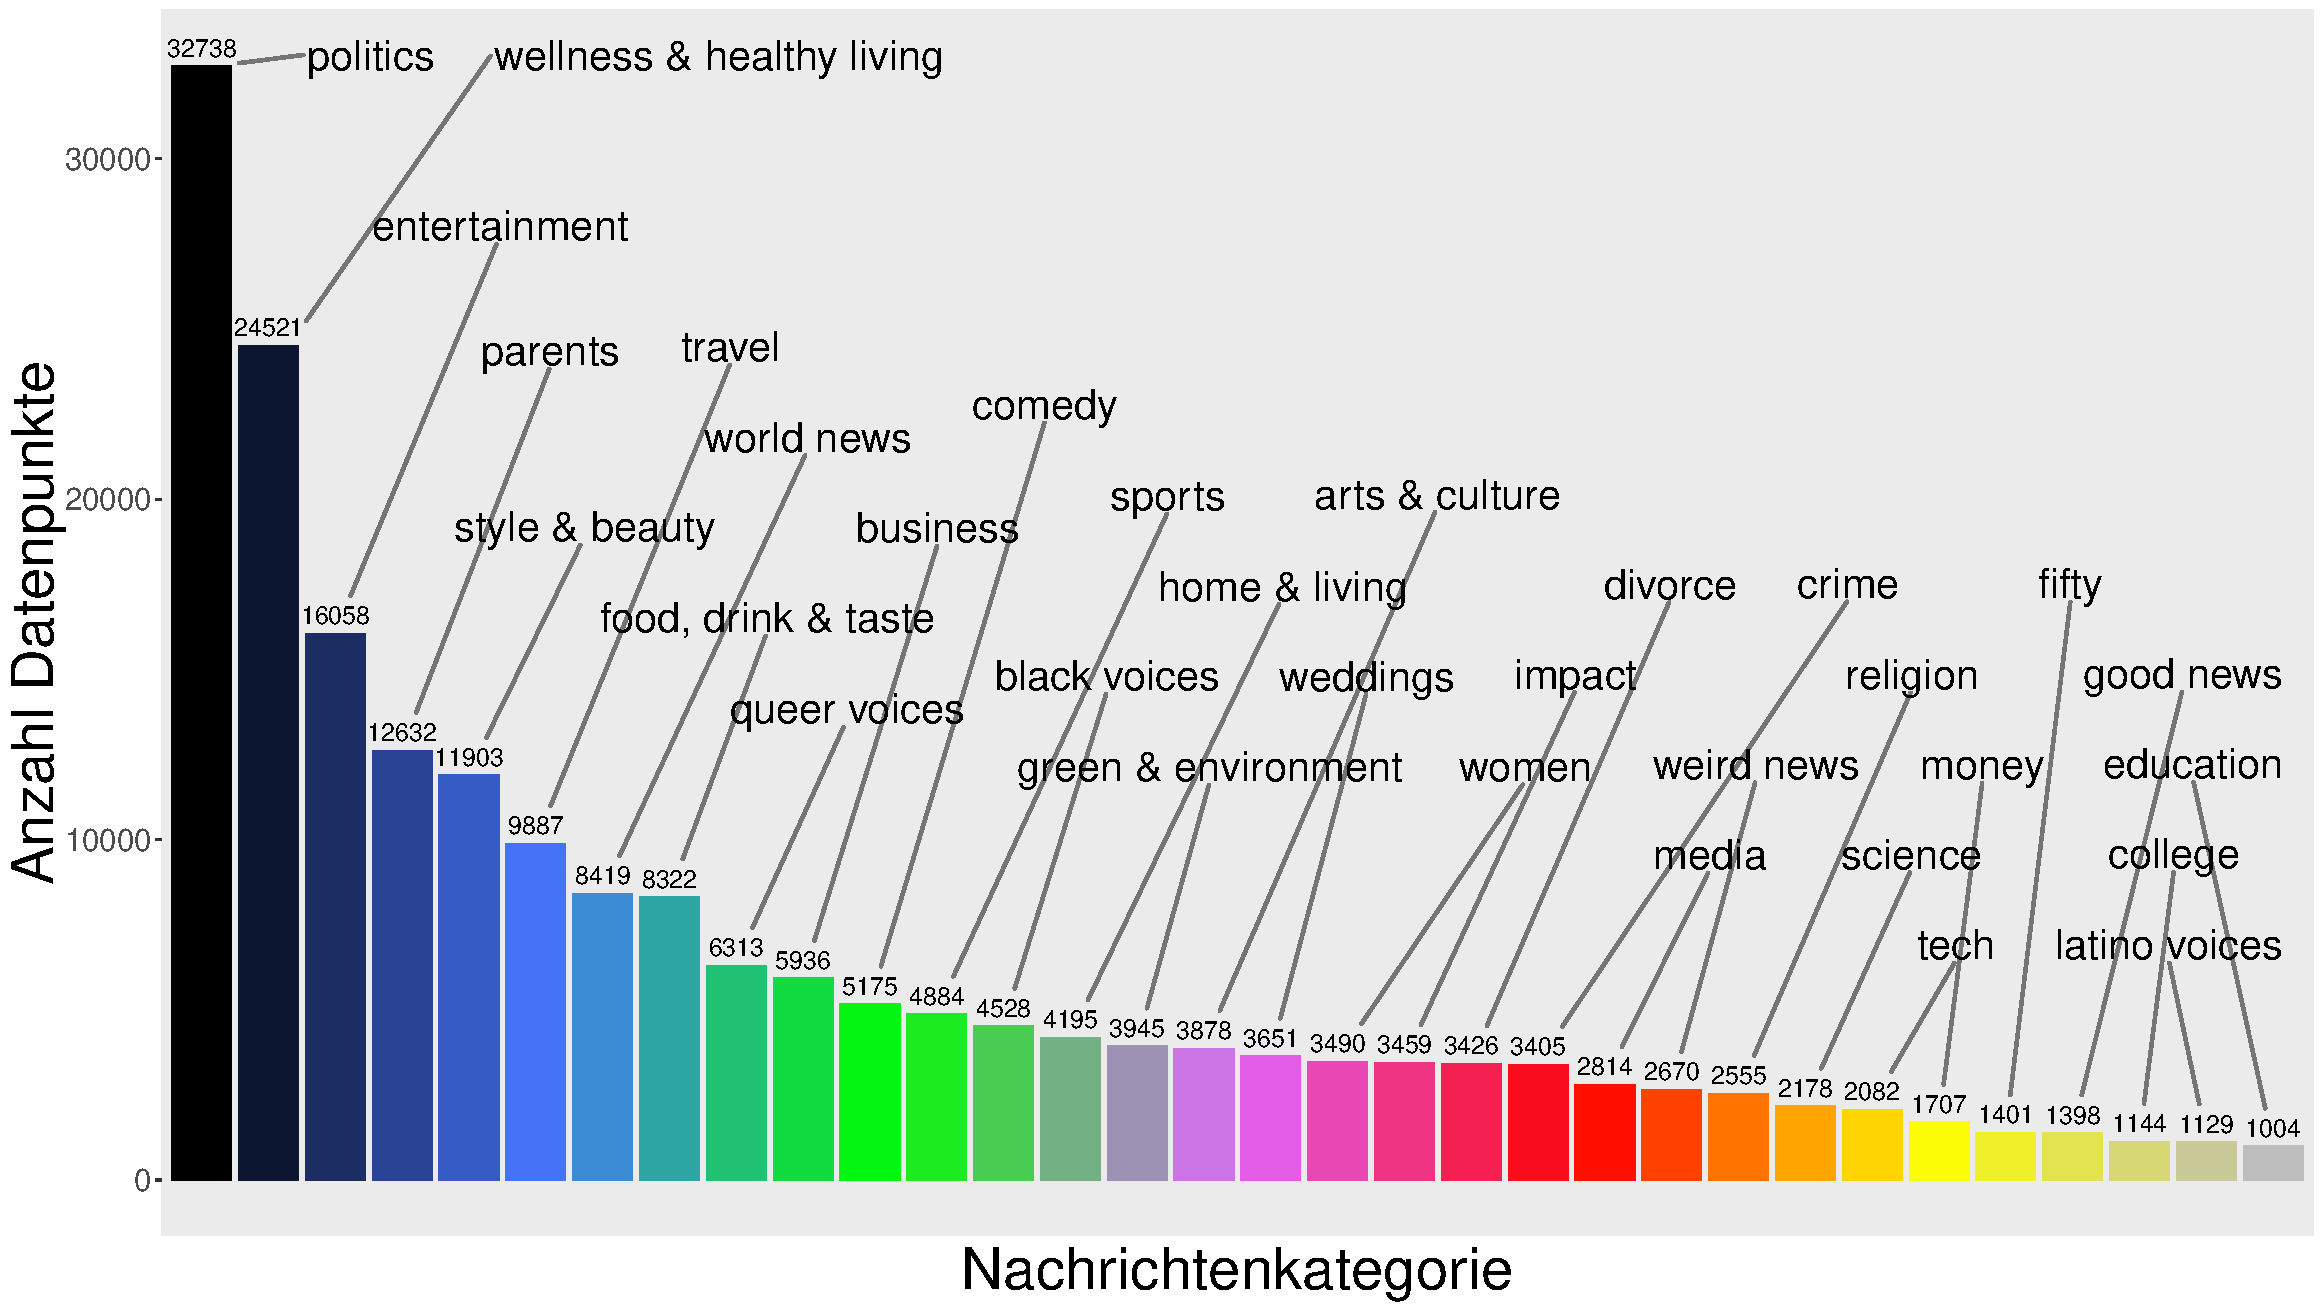
\includegraphics[width = \textwidth,  keepaspectratio]{Images/barplotCategories.pdf} 
\label{abb:barplotCategories}
\caption{Anzahl Datenpunkte pro Nachrichtenkategorie}
\end{figure}
todo: box um die labels größer machen.\\

Es ist festzustellen, dass die Kategorien keineswegs ausgeglichen vorliegen. Die häufigste Kategorie stellt \textit{politics} dar mit $32738$ Datenpunkten. Zweit- und dritthäufigste Kategorien sind \textit{wellness} und \textit{entertainment} mit $17827$ und $16058$ Beobachtungen. Die Nachrichtensparten mit den wenigsten Artikeln bilden \textit{college}, \textit{latino voices} und \textit{education} mit $1144$, $1129$ und $1004$ Beobachtungen.\\
Die ersten $6$ Kategorien stellen bereits $50.3$ Prozent der gesamten Beobachtungen dar. Durchschnittlich beinhaltet eine Kategorie $5738.5$ Nachrichtenschlagzeilen.\\
\\
Es folgt nun eine gesamtheitliche Exploration des Textkorpus der Schlagzeilen. Im Rahmen der Analyse zählen Symbole sämtlicher Art auch als Wörter. Die kürzeste Überschrift des Datensatzes enthält nur $1$ Wort, während die längste $91$ Wörter umfasst. Durchschnittlich enthält eine Schlagzeile $11.147$ Wörter. Das Vokabular aller Schlagzeilen umfasst $67938$ Wörter, wobei \say{the} das häufigste Wort ist und in $54033$ Artikelüberschriften vorkommt. $31274$ Wörter kommen nur einmal vor. In der Betrachtung der mittleren Wortanzahlen pro Kategorie fällt auf, dass diese differieren. Die Kategorie mit der höchsten durchschnittlichen Anzahl von $12.863$ Wörtern ist \textit{style \& beauty}. Die Kategorie, bei der sich die Autoren durchschnittlich am kürzesten fassen, ist \textit{food \& drink} mit $9.328$ Wörtern. Eine weitere interessante Fragestellung ist, ob in den Kategorien bestimmte Sonderzeichen oder Symbole besonders häufig oder selten vorkommen. Abbildung \ref{abb:barplotSymbols} zeigt die relative Anzahl der Vorkommnisse verschiedener Symbole in den Schlagzeilen pro Kategorie.

\begin{figure}[ht]
    \centering
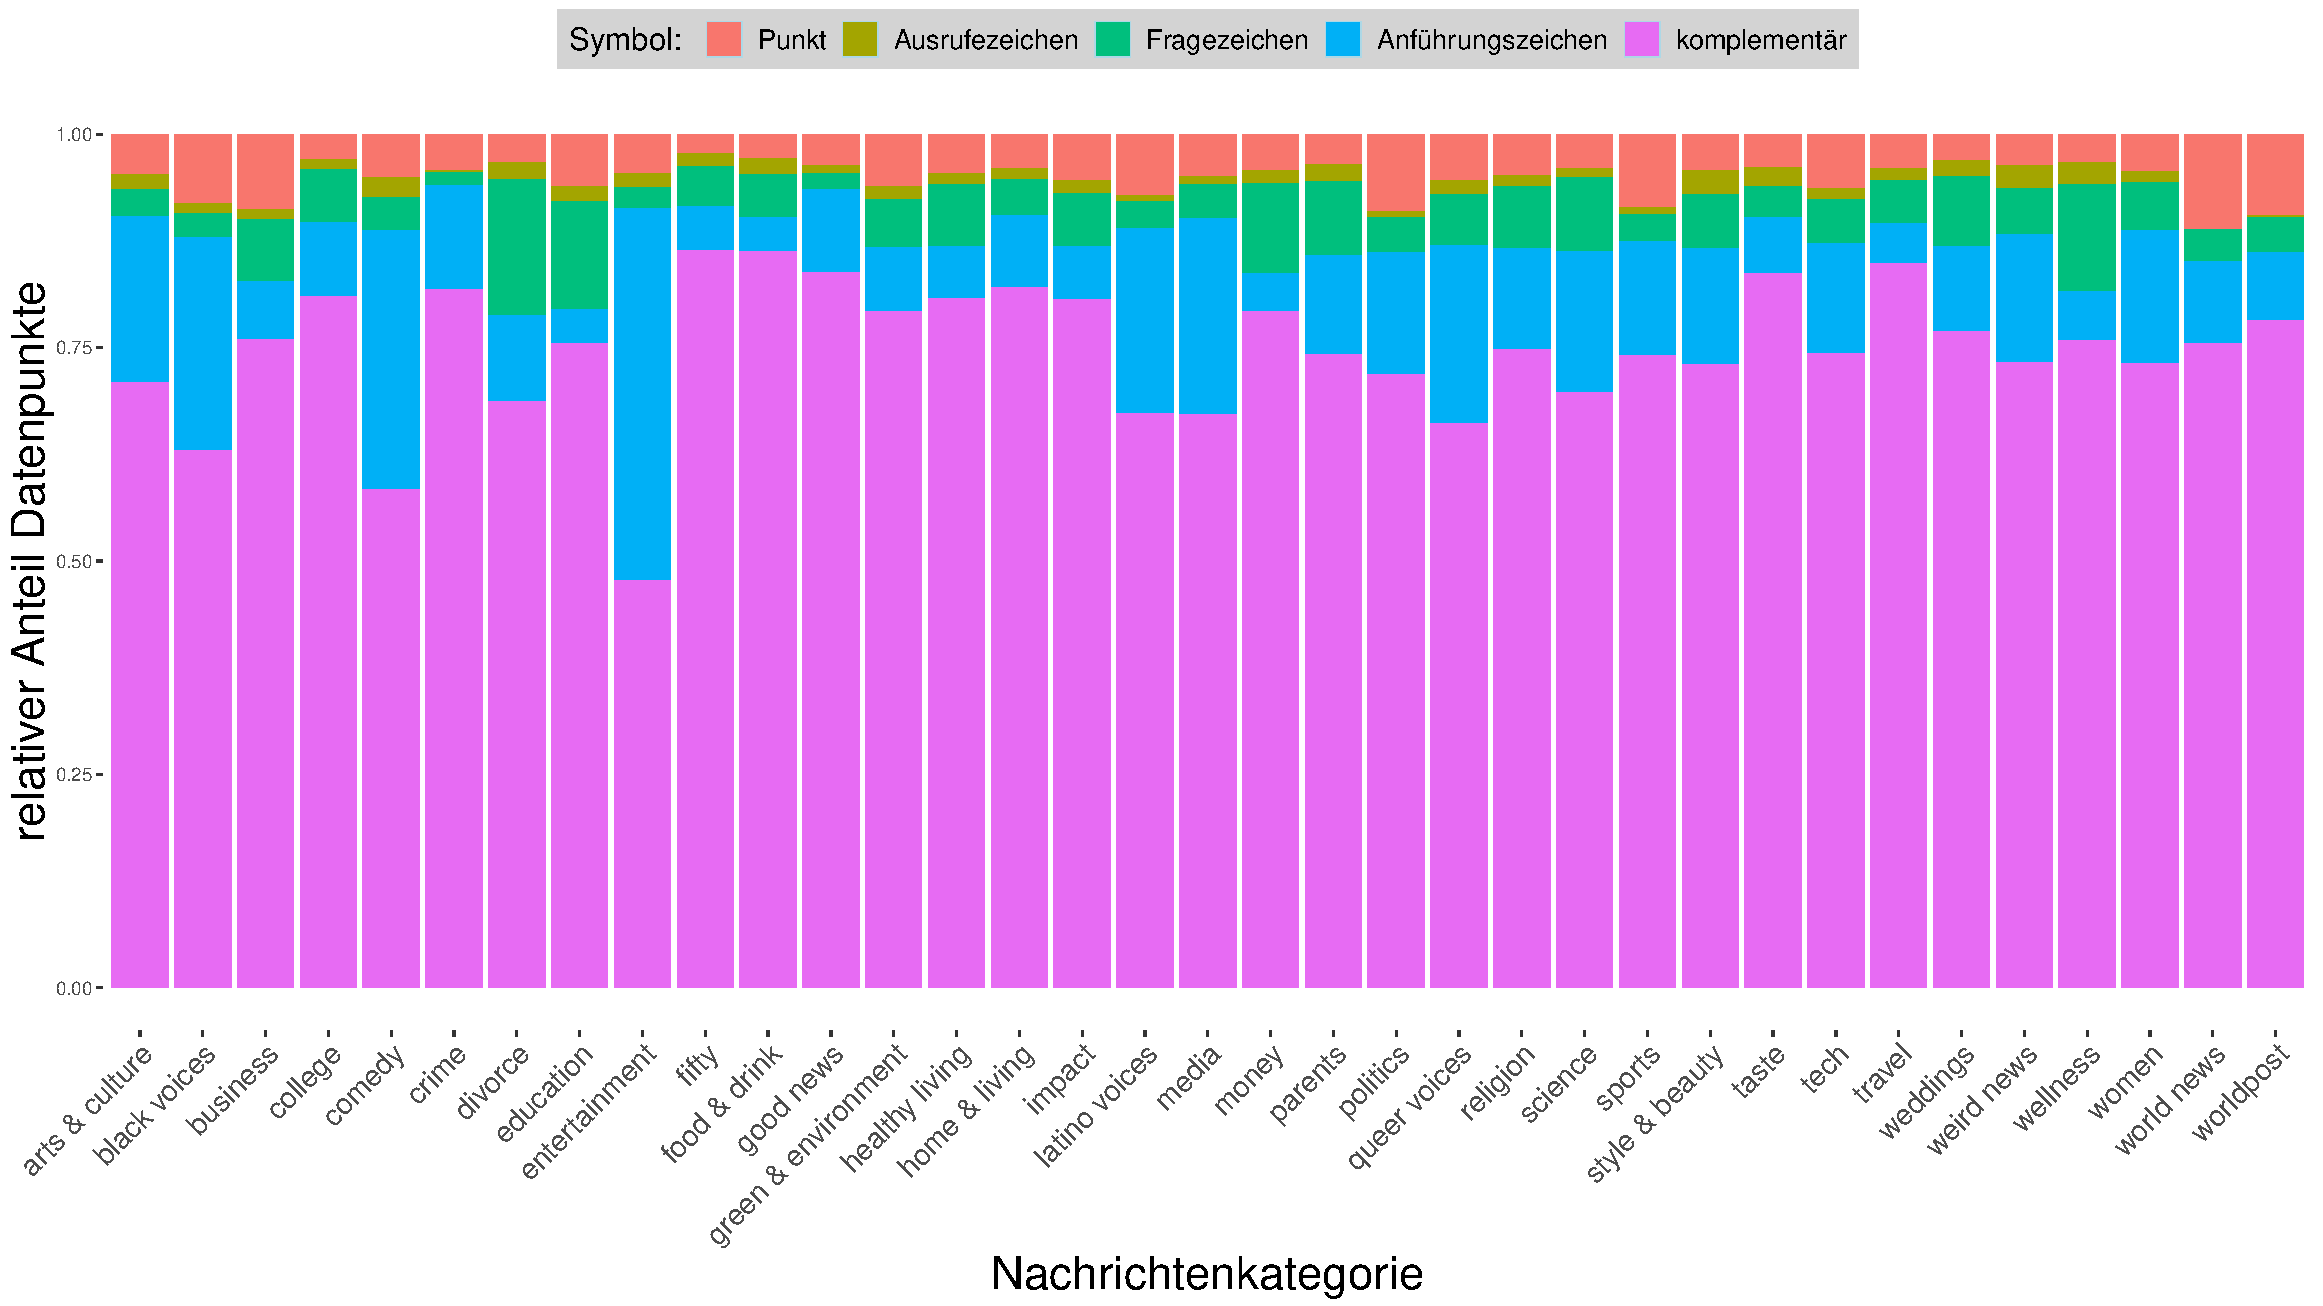
\includegraphics[width = \textwidth,  keepaspectratio]{Images/barplotSymbols.pdf} 
\label{abb:barplotSymbols}
\caption{Relativer Anteil Datenpunkte mit Sonderzeichen pro Kategorie}
\end{figure}

Ein Wert von beispielsweise $0.15$ für eine bestimmte Nachrichtensparte in der Grafik ist so zu interpretieren, dass in 15 Prozent aller Schlagzeilen dieser Kategorie das entsprechende Symbol mindestens einmal aufgetaucht ist. Die im Folgenden beschriebenen Durchschnitte sind Mittelwerte über die Kategorien und nicht über den gesamten Datensatz. Betrachtet sei nun das Vorkommen eines Punktes in einer Schlagzeile. Dieses kann so interpretiert werden, dass eine Schlagzeile 2
mehrere Sätze enthält. Dies ist insgesamt mit einem durchschnittlichen relativen Anteil von $0.051$ selten der Fall. In der Sparte \textit{world news} kommen mehrere Sätze am häufigsten vor, in \textit{fifty} am wenigsten. Der Mittelwert für Ausrufezeichen beträgt $0.014$ und die Kategorie \textit{style \& beauty} nimmt das Maximum, die Kategorie \textit{world news} das Minimum an. Fragezeichen kommen in durchschnittlich $0.059$ der Schlagzeilen vor, dabei am häufigsten in \textit{divorce} und am seltensten in \textit{crime}. Anführungszeichen sind mit durchschnittlich $0.127$ von den hier betrachteten Satzzeichen am meisten vertreten. Sie wurden besonders oft in der \textit{entertainment} Sparte genutzt und kamen am seltensten in \textit{education} zum Einsatz. Die Rubrik \say{komplementär} gibt an, zu welchem relativen Anteil keine der betrachteten Symbole vorkommt. Hier ist zu sehen, dass Kategorien wie \textit{entertainment}, \textit{comedy}, \textit{black voices} oder \textit{divorce} häufig Symbole beinhalten, die einen dramatischen Charakter ausdrücken. Sparten wie \textit{fifty}, \textit{food \& drink} und \textit{travel} bleiben mit weniger Symbolen sachlicher. Abbildung \ref{abb:barplotSymbols} zeigt insgesamt, dass Symbole für die Nachrichtensparten eine Rolle spielen und für die in Kapitel \ref{Kap:Bow} und \ref{Kap:Tfidf} beschriebenen \textit{bag-of-words} und \textit{tfidf} (todo, hier entfernen, falls die Algos doch nicht genutzt werden) Ansätze nicht entfernt werden sollten.\\
\\
Es folgt nun eine Betrachtung der vorkommenden Wörter im Datensatz. Abbildung \ref{abb:WordcloudAll} zeigt eine \textit{wordcloud}, in der die häufigsten $100$ Wörter aller Kategorien (nach Entfernung von Symbolen und \textit{stopwords}) abgebildet sind.

\begin{figure}[ht]
    \centering
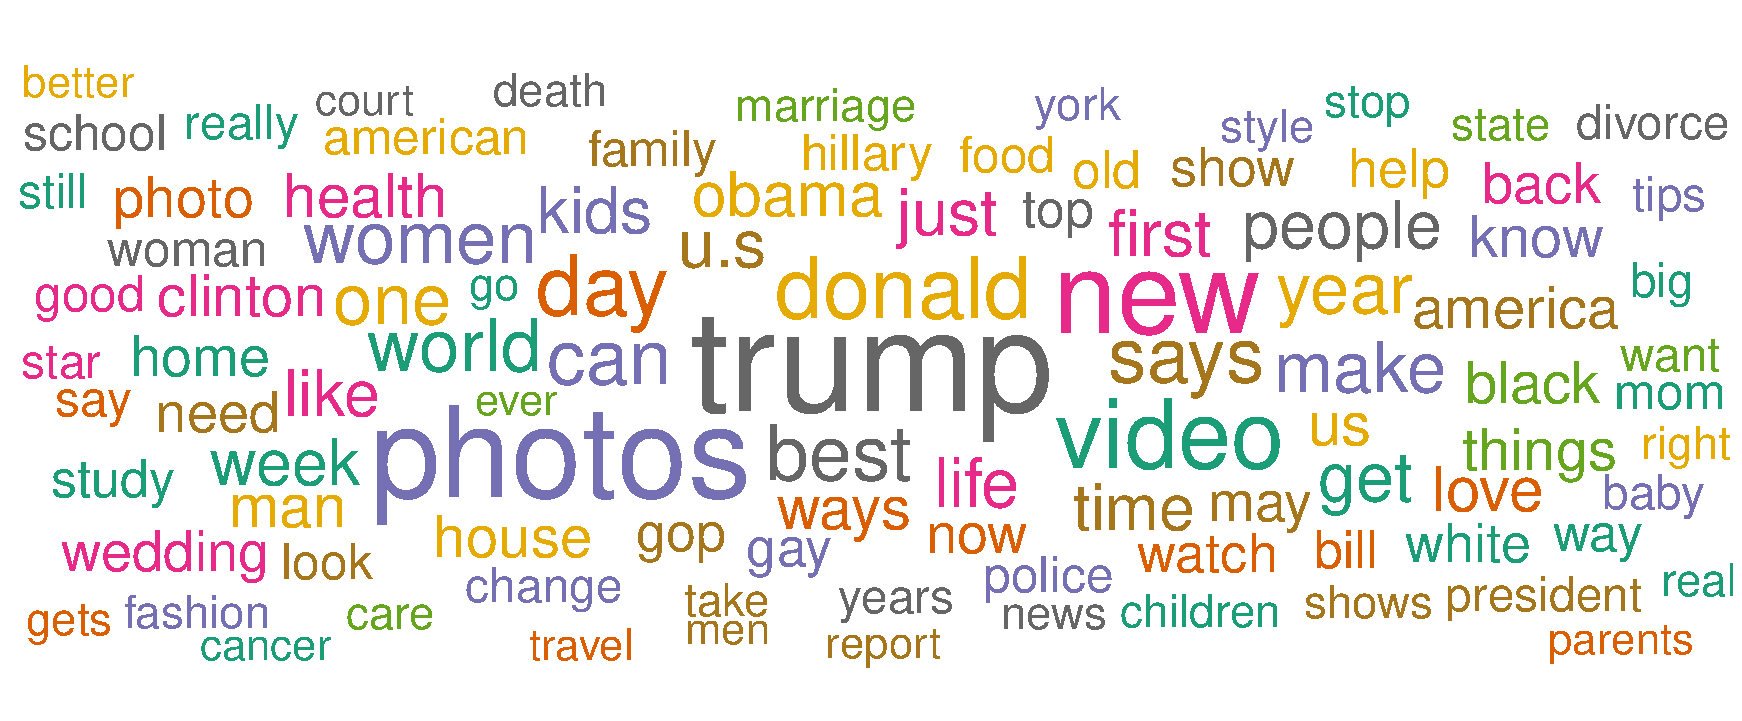
\includegraphics[width = \textwidth,  keepaspectratio]{Images/wordCloudAll.pdf} 
\label{abb:WordcloudAll}
\caption{\textit{Wordcloud} für die häufigsten 100 Wörter aller Kategorien}
\end{figure}
todo: grafik gescheit ausfüllen

Je größer ein Wort, desto häufiger kommt es insgesamt im Textkorpus vor. Es ist erstaunlich, dass \say{trump} sich über den gesamten Textkorpus als häufigstes Wort etabliert hat, in Anbetracht dessen, dass sich der Zeitraum der Daten auf über $6$ Jahre erstreckt. Die $3$ häufigsten Wörter danach sind \say{photos}, \say{new} und \say{video}. Es ist zu sehen, dass viele Namen und Begriffe aus der Politik zu sehen sind, was einleuchtend ist, da \textit{politics} zu größte Sparte darstellt. 
Auffallend ist außerdem, dass viele der auftauchenden Begriffe identisch oder fast identisch zu den Namen einiger Kategorien sind. Beispiele dafür sind \say{travel}, \say{wedding}, \say{style} oder \say{parents}. In Abbildung \ref{abb:WordcloudWellness} ist eine weitere \textit{Wordcloud} der zweitgrößten Sparte \textit{wellness} zu sehen.


\begin{figure}[ht]
    \centering
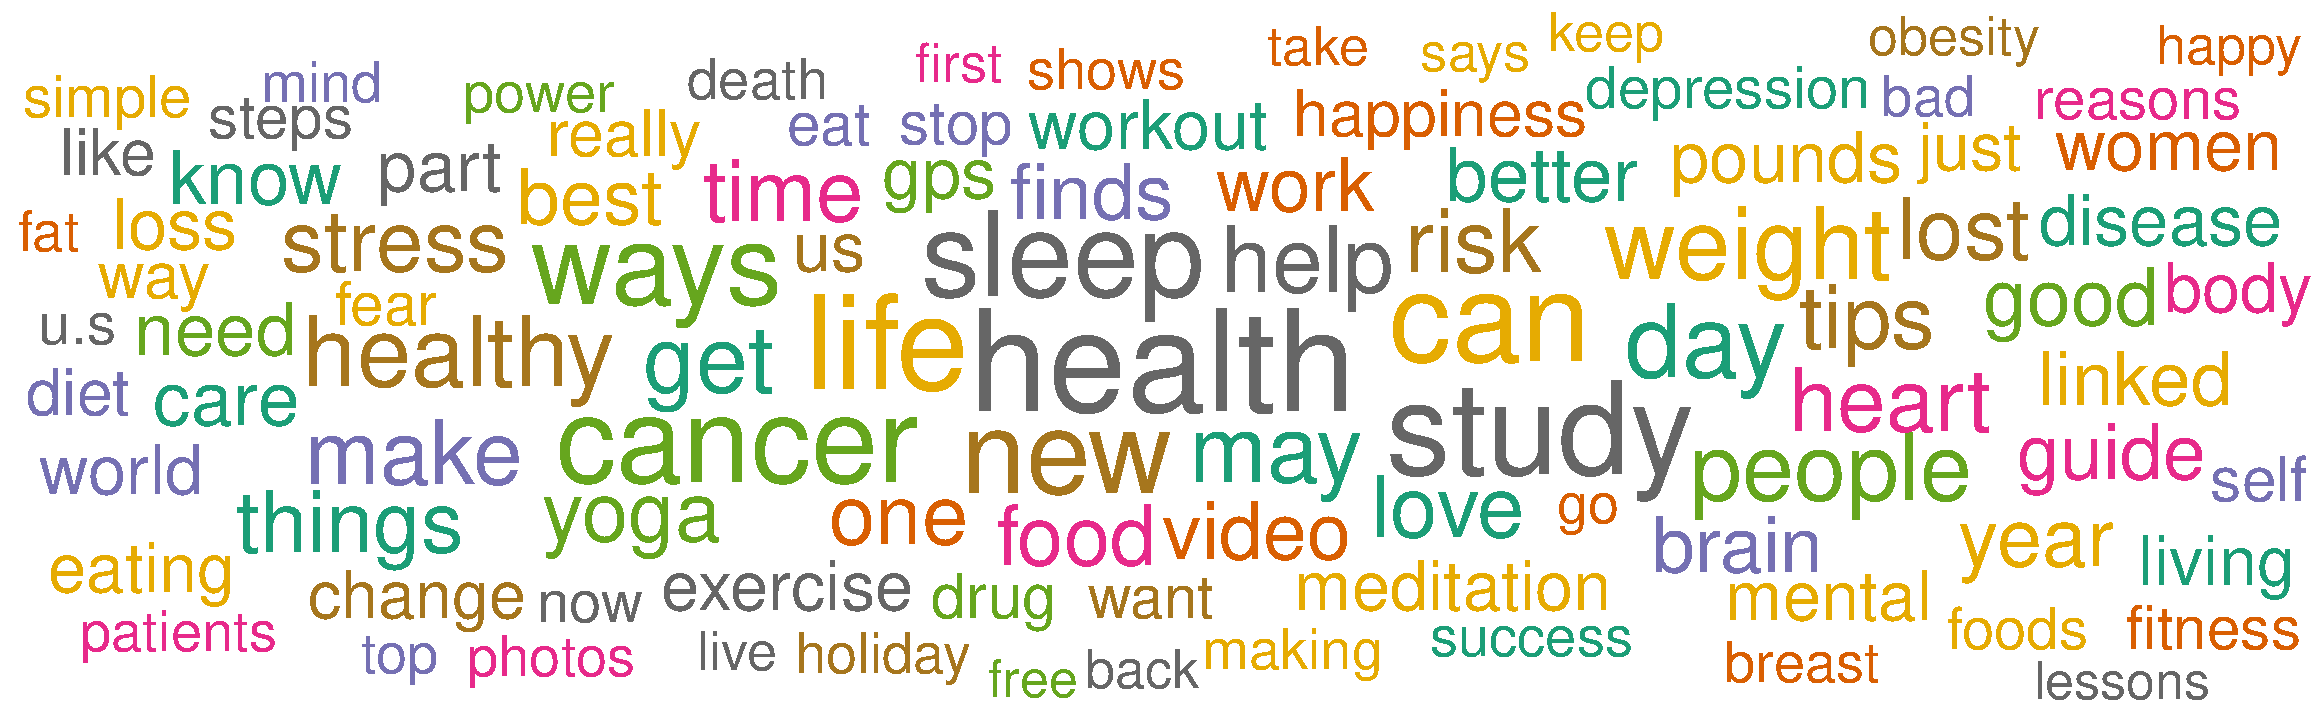
\includegraphics[width = \textwidth,  keepaspectratio]{Images/wordCloudWellness.pdf} 
\label{abb:WordcloudWellness}
\caption{\textit{Wordcloud} für die häufigsten 100 Wörter der Kategorie \textit{wellness}}
\end{figure}

In dieser Kategorie ist zu beobachten, dass oft über Schlaf, Yoga, Meditation und Sport geschrieben wird. Es werden aber auch Krankheiten wie Krebs (\say{cancer}), Übergewichtigkeit (\say{obesity}) und Diabetis angesprochen, die genauso für die Kategorie \textit{healthy living} stehen könnten. \say{yoga}, \say{breast}, \say{diet} oder \say{pounds} könnten auch legitime Schlagwörter für die \say{women} Sparte sein. Genauso ist zu vermuten, dass die Wörter \say{eat}, \say{foods} und \say{healthy} ebenso in \say{food \& drink} oft vorzufinden sind. Mit dem Blick auf die \textit{Wordclouds} und auch in Anbetracht der Kategorienzusammenlegung in Kapitel \ref{kap:2_2Aend} fällt auf, dass es nicht immer einfach ist, die Kategorien nur über ihre häufigsten Schlagwörter auseinanderzuhalten. Auf die verschiedenen Möglichkeiten, wie die Schlagzeilen in ein numerisches Datenformat überführt werden können, wird in Kapitel \ref{kap:3.1Wordemb} detailiert eingegangen.
Nachdem nun der Datensatz ausführlich exploriert wurde, folgt im nächsten Unterabschnitt die Zielstellung dieser Thesis.


\subsection{Zielstellung} \label{Kap:Zielst}

Ziel dieser Arbeit soll es sein, verschiedene Algorithmen auf verschiedenen Arten der Repräsentation der Wörter miteinander zu vergleichen. Dabei liegt ein \textit{multilabel}-Klassifikations\-problem mit $35$ Klassen vor, bei der jede Beobachtung genau einer Klasse zugehörig ist. Die Zielvariable liegt im kategoriellen Format vor. Dabei soll für die Vorhersagen $f(x_i)$ der trainierten Modelle gelten, dass
\begin{center}
$f(x_i) = p_i = (p(c_1), ...., p(c_{35}))$ \hspace{2cm} , mit $\sum\limits_{i = 1}^{35} p(c_i) = 1 $,
\end{center}
dabei sind $p(c_j)$, $j = 1,...,35$ die modellierten Wahrscheinlichkeiten der Zugehörigkeit der Beobachtung $x_i$ zur Klasse $c_j$, die in Summe $1$ ergeben müssen. Die eindeutige prognostizierte Klasse $\hat{y}$ wird dann zugeordnet durch 
\begin{center}
    $\hat{y_i} =  \underset{c_1,...,c_{35}}{argmax}$ $p(c_j)$.
\end{center}

Bezüglich der Güte der Modelle soll dann mit den Gütemaßen aus Kapitel \ref{kap:guetemass} ein Vergleich erfolgen. Dabei ist nicht nur von Interesse, wie gut die Modelle insgesamt abschneiden, sondern auch ob manche Modelle bestimmte Kategorien trennschärfer identifizieren können und welche Gründe es dafür gibt. Des Weiteren soll analysiert werden, in welche Nachbarklassen die Beobachtungen bei einer Fehlklassifikation eingeordnet werden und ob diese inhaltlich nahe an der richtigen Kategorie ist. Eine weitere Untersuchungsfrage für die Modellgüte ist, inwiefern die Repräsentation der Wörter ausschlaggebend sind und welches Gewicht der verwendete Algorithmus dabei einnimmt.
Nun sollen im nächsten Abschnitt die statistischen Methoden beschrieben werden.
(todo: diesen Abschnitt im Laufe der Arbeit ergänzen)

\newpage

\section{Statistische Methoden}

Dieses Kapitel ist in $3$ Abschnitte unterteilt. Zuerst werden die zur Bewertung der Modelle herangezogenen Gütemaße beschrieben. Es folgt die Darlegung der verschiedenen Methoden zur numerischen Repräsentation von Wörtern. Zuletzt folgt die ausführliche Beschreibung der in dieser Arbeit benutzten \textit{machine-learning} Algorithmen.

\subsection{Gütemaße zur Evaluation der Modelle}\label{kap:guetemass}

Eine Bewertung der Modelle erfolgt dann über verschiedene Kennzahlen. Einige davon werden unter Verwendung der \textit{confusion matrix} (oder auch Klassifikationsmatrix) berechnet. Diese in Tabelle \ref{tab:confusionMatrix} zu sehende Matrix stellt nach dem Anwenden des Modells auf den Testdatensatz die resultierenden Richtig- und Falschklassifikationen übersichtlich dar.

\begin{table}[ht]
\begin{center}
\begin{tabular}{|c|ccc|c|}
  \hline
 & \multicolumn{3}{|c|}{Prognostizierte Klasse} &  \\
Wahre Klasse & Kategorie $c_1$ & ...  & Kategorie $c_n$ & Zeilensumme  \\ 
  \hline
Kategorie $c_1$ & $h_{11}$ & $\hdots$ & $h_{1n}$ & $\sum_{j=1}^n h_{1j}$\\
$\vdots$ & $\vdots$ & $\ddots$ & $\vdots$ & $\vdots$ \\
Kategorie $c_n$ & $h_{n1}$ & $\hdots$ & $h_{nn}$ & $\sum_{j=1}^n h_{nj}$\\
\hline
Spaltensumme & $\sum_{i=1}^n h_{i1}$ & $\vdots$ & $\sum_{i=1}^n h_{in}$ & 
$N = \sum_{i=1}^n \sum_{j=1}^n h_{ij}$\\
   \hline
\end{tabular}
\label{tab:confusionMatrix}

  \caption{Übersicht über eine \textit{confusion matrix}  für $n$  Klassen (vgl. \cite{backhaus}, S. 238)}  
\end{center}
\end{table}

Die absoluten Häufigkeiten $h_{ij}$ stehen für die Anzahl der Beobachtungen aus der wahren Klasse $i$, für die die Klasse $j$ prognostiziert wurde. Aus der \textit{confusion matrix} können folgende Größen identifiziert werden. Die \textit{true-positives} der Klasse $i$, $tp_i = h_{ii}$ sind alle Beobachtungen, die Klasse $i$ zugehörig sind und auch in selbige Klassifiziert wurden. Die Beobachtungen, die in Klasse $i$ klassifiziert wurden, aber einer anderen wahren Klasse zugehörig sind, bezeichnet man als \textit{false-positives} $fp_i = \sum_{j = 1}^n h_{ji} - h{ii}$. Als \textit{true-negatives} $tn_i \sum_{j = 1}^n h_{ij} - h{ii}$ werden die Beobachtungen bezeichnet, die der Klasse $i$ zugehörig sind, aber in eine andere Kategorie falsch klassifiziert werden. Letztlich sind \textit{false-negatives} $fn_i = N - (tp_i + fp_i + tn_i)$ die Datenpunkte, die nicht Kategorie $i$ angehören und für die auch nicht in $i$ prognostiziert wird (vgl. \cite{sokolova}). Unter Kenntnis der 4 Häufigkeiten können nun verschiedene Gütemaße dargelegt werden. 


Die \textit{accuracy} berechnet sich analog zur binären Klassifikation aus 
\[ Acc = \frac{\sum_{i=1}^n tp_i}{N} \],
ist also der Anteil der richtig klassifizierten Beobachtungen an allen Beobachtungen. Dieses Maß ist jedoch gerade bei unbalancierten Klassifikationsproblemen nicht ideal, da große Klassen stark favorisiert werden und ein Modell schon eine hohe Güte erzielen kann, indem es alle Beobachtungen der größten Klasse zuordnet (todo quelle finden). Es folgen die Maße \textit{precision}, \textit{recall} und darauf aufbauende Kennzahlen, welche bei unterschiedlichen Klassengrößen geeigneter sind. Es wird von einer hohen \textit{precision} der Klasse $i$gesprochen, wenn nach Prognose in Klasse $i$ ein hoher Anteil dieser Beobachtungen auch tatsächlich aus derselben Kategorie stammt. Wiederum hat das Modell bezüglich Klasse $i$ einen hohen \textit{recall}, falls von den Beobachtungen der Klasse $i$ auch ein hoher Anteil in Klasse $i$ eingeordnet wird.
In der \textit{multiclass}-Klassifikation kann ein Gütemaß für das komplette Modell über \textit{micro-averaging} (mit $\mu$ indiziert) oder \textit{macro-averaging} (mit $M$ indiziert) berechnet werden. Es sind dann 
\[ precision_{\mu} = \frac{\sum_{i = 1}^n tp_i}{\sum_{i = 1}^n (tp_i + fp_i)}, \hspace{1cm} recall_{\mu} = \frac{\sum_{i = 1}^n tp_i}{\sum_{i = 1}^n (tp_i + fn_i)}\],
\[ precision_M = \frac{\sum_{i = 1}^n \frac{tp_i}{tp_i + fp_i} }{l}, \hspace{1cm} recall_M = \frac{\sum_{i = 1}^n \frac{tp_i}{tp_i + fn_i} }{l}\]
die Maße für das gesamte Modell. Ein Maß, dass \textit{precision} und \textit{recall} kombiniert ist der \textit{fscore}. Mit der unterschiedlichen Durchschnittsbildung ergeben sich
\[ fscore_{\mu} = \frac{(\beta^2+1) precision_{\mu} recall_{\mu}}{\beta^2 precision_{\mu}+ recall_{\mu}}, \hspace{1cm} fscore_{M} = \frac{(\beta^2+1) precision_{M} recall_{M}}{\beta^2 precision_{M}+ recall_{M}} \].
Hierbei ist anzumerken, dass $fscore_{\mu}$ Klassen mit vielen Beobachtungen in der Güte begünstigt während für $fscore_M$ alle Kategorien gleich wichtig sind.(todo: $beta$ spezifizieren oder multiclass AUC beschreiben).  In der statistischen Auswertung in Kapitel \ref{Kap:statAus} werden beide Kennzahlen zur Bewertung der Modelle herangezogen.

\begin{itemize}
    \item mlogloss/cross entropy, damit nachbarklassen nicht stark bestraft werden
\end{itemize}{}

\subsection{Repräsentationen der Wörter und Sätze (mit preprocessing der tokens} \label{kap:3.1Wordemb}
\subsubsection{Bag-Of-Words} \label{Kap:Bow}
\subsubsection{Term Frequency Inverse Document frequency} \label{Kap:Tfidf}
\subsubsection{Sequentielle Darstellung}
\subsubsection{Word-To-Vec Überwacht, Summe von Word-To-Vec}
\subsubsection{Glove Embeddings} \label{Kap:Glove}


\subsection{Algorithmen und Verfahren}

\subsubsection{Extreme Gradient Boosting}
\subsubsection{Random Forest}
\subsubsection{Neuronales Netz: Multi-Layer-Perception}
\subsubsection{Neuronales Netz: Convolutional Neural Net}
\subsubsection{Neuronales Netz: Long-Short-Term-Memory Neural Net}

\begin{itemize}
    \item grafik über kombination von word embeddings und Algorithmen (was kann mit was verwendet werden)
\end{itemize}{}


\section{Statistische Auswertung}\label{Kap:statAus}

\subsection{Vorauswahl der Verfahren}

\begin{itemize}
    \item grafik mit framework zu train/test/validation (10 prozent vorauswahl benchmarken, dann auf 90 prozent traintest/tuning. Die selben Modelle dann auf 10 prozent valdata validieren? 10 prozent war, weil dann in der kleinsten klasse noch mindestens $100$ Beobachtungen sind.
    \item außerdem welche tokens entfernt wurden.
    \item tabelle mit allem was ich ausprobiert habe
\end{itemize}{}

\subsection{Anwendung der Modelle}
\subsubsection{Performanzmaße}

\begin{itemize}
    \item accuracy, mse etc
    \item accuracy by class comparison
    \item confidence vs accuracy plots
    \item maß wie sicher ist sich das Verfahren, wenn es die richtige klasse ist?
\end{itemize}{}

\subsubsection{Explaining der besten Modelle}

\begin{itemize}
    \item beobachtungen verändern, wörter wegnehmen, hinzufügen, reihenfolge ändern und schauen ob das verfahren stabil /sensitiv zur reihenfolge
    \item nachbarklassen identifizieren
    \item convolutional filters holen und ähnlichkeiten zu combinationen aus word vectors erhalten
\end{itemize}{}

\subsubsection{Anpassung des besten Modell auf den gesamten Datensatz}

\section{Zusammenfassung}

\subsection{Ergebnisse}
\subsection{Fazit und Ausblick}

\newpage

\printbibliography[
heading=bibintoc,
title={Literaturverzeichnis}
]


\end{document}


